%%%%%%%%%%%%%%%%

% designed to be integrated with conceptual figure

%%%%%%%%%%%
\documentclass[border=0.2cm,11pt]{standalone}
\usepackage{tgheros}
\renewcommand*\familydefault{\sfdefault}%

\usepackage{tikz}
\usetikzlibrary{positioning,automata}
\usetikzlibrary{shapes}

\tikzset{>=latex} % for LaTeX arrow head
\usepackage{xcolor}

% taken from neural networks
\usepackage{amsmath} % for aligned
%\usepackage{amssymb} % for \mathbb
%\usepackage{etoolbox} % for \ifthen
\usepackage{listofitems} % for \readlist to create arrays
\usetikzlibrary{arrows.meta} % for arrow size
\usepackage[outline]{contour} % glow around text
\contourlength{1.4pt}

% using tableau 10 color palette: https://public.tableau.com/views/TableauColors/ColorPaletteswithRGBValues?%3Aembed=y&%3AshowVizHome=no&%3Adisplay_count=y&%3Adisplay_static_image=y

\definecolor{myblue}{RGB}{31,119,180}
\definecolor{myred}{RGB}{214,39,40}
\definecolor{mygreen}{RGB}{44,160,44}

% original colors defined by original author
\colorlet{myorange}{orange!70!red!60!black}
\colorlet{mydarkred}{red!30!black}
\colorlet{mydarkblue}{blue!40!black}
\colorlet{mydarkgreen}{green!30!black}
\tikzstyle{mynode}=[align=center, rounded corners, minimum height=1cm]
\tikzstyle{procs_ecolo}=[mynode, rectangle, fill=mygreen!30]
\tikzstyle{procs_evol}=[mynode, rectangle, fill=myred!30]
\tikzstyle{mechanisms}=[mynode, rectangle, thick, minimum width=3cm]
\tikzstyle{patterns}=[mynode, circle, thick, fill=myblue!20]
\tikzstyle{node_cust}=[minimum height=1cm, minimum width=3.5cm, fill=black!10,rounded corners,draw=black!30]


% \tikzstyle{node}=[ultra thick,circle,minimum size=30,inner sep=2.,outer sep=0.6]
% \tikzstyle{node green}=[node,fill=mygreen]
% \tikzstyle{node blue}=[node,fill=myblue]
% \tikzstyle{node orange}=[node,orange!20!black,draw=myorange!30!black,fill=myorange!20]
% \tikzstyle{node red}=[node,fill=myred]
\tikzstyle{connect}=[thick,mydarkblue] %,line cap=round
\tikzstyle{connect arrow}=[-{Latex[length=6,width=6]},thick,mydarkblue,shorten <=0.5,shorten >=1]
 

% spacing nodes
% \tikzset{node distance = 0.5cm and 0.5cm}

\begin{document}

 
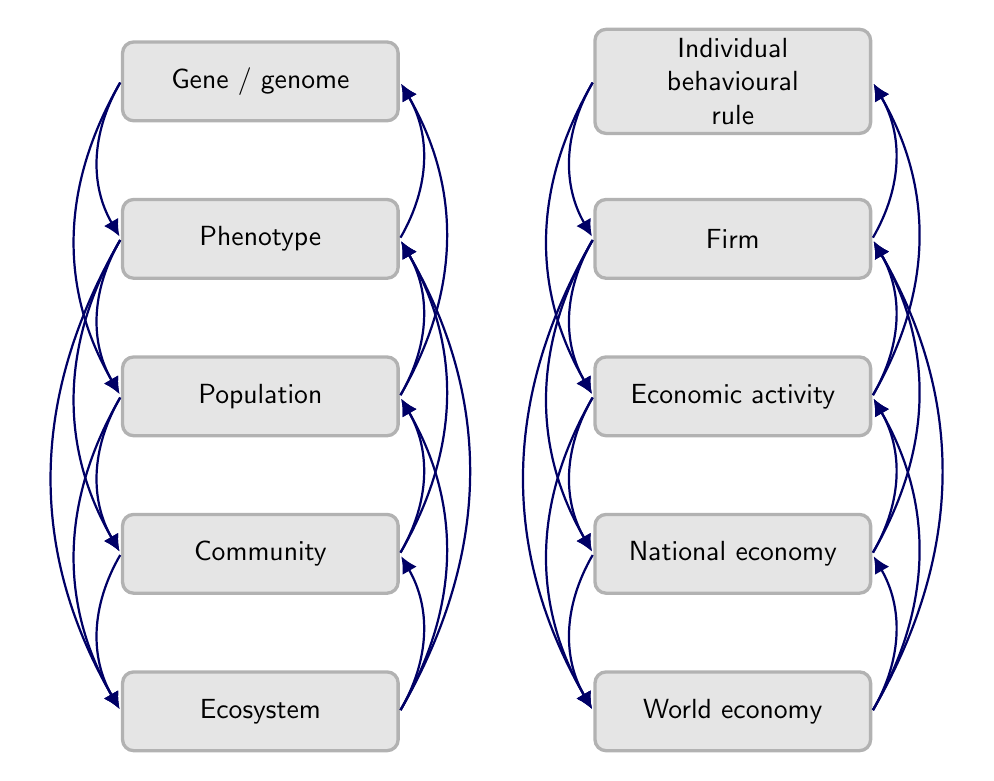
\begin{tikzpicture}[
    node distance=2cm,
    on grid,
    very thick]

% biological systems
        \node[node_cust, align=center] (genes) {Gene / genome};
        \node[node_cust, below=of genes] (phen) {Phenotype};
        \node[node_cust, below=of phen] (pop) {Population};
        \node[node_cust, below=of pop] (com) {Community};
        \node[node_cust, below=of com] (ecos) {Ecosystem};
        % biological systems
        \node[node_cust,right=6cm of genes,align=center] (orga) {Individual\\behavioural\\rule};
        \node[node_cust,below=of orga] (Firms) {Firm};
        \node[node_cust,below=of Firms] (ecoa) {Economic activity};
        \node[node_cust,below=of ecoa] (nateco) {National economy};
        \node[node_cust,below=of nateco] (weco) {World economy};

        \begin{scope}[connect arrow]
            \draw (genes.west) to [bend right] (phen.west);
            \draw (genes.west) to [bend right] (pop.west);

            \draw (phen.west)  to [bend right] (pop.west);
            \draw (phen.west)  to [bend right] (com.west);
            \draw (phen.west)  to [bend right] (ecos.west);
            \draw (pop.west)   to [bend right] (com.west);
            \draw (pop.west)   to [bend right] (ecos.west);
            \draw (com.west)   to [bend right] (ecos.west);
            \draw (phen.east)  to [bend right] (genes.east);

            \draw (ecos.east) to [bend right] (com.east);
            \draw (ecos.east) to [bend right] (pop.east);
            \draw (ecos.east) to [bend right] (phen.east);
            \draw (com.east) to [bend right] (pop.east);
            \draw (com.east) to [bend right] (phen.east);
            \draw (pop.east) to [bend right] (phen.east);
            \draw (pop.east) to [bend right] (genes.east);

        \end{scope}

        \begin{scope}[connect arrow]
            \draw (orga.west) to [bend right] (Firms.west);
            \draw (orga.west) to [bend right] (ecoa.west);

            \draw (Firms.west)  to [bend right] (ecoa.west);
            \draw (Firms.west)  to [bend right] (nateco.west);
            \draw (Firms.west)  to [bend right] (weco.west);
            \draw (ecoa.west)   to [bend right] (nateco.west);
            \draw (ecoa.west)   to [bend right] (weco.west);
            \draw (nateco.west)   to [bend right] (weco.west);
            \draw (Firms.east)  to [bend right] (orga.east);

            \draw (weco.east) to [bend right] (nateco.east);
            \draw (weco.east) to [bend right] (ecoa.east);
            \draw (weco.east) to [bend right] (Firms.east);
            \draw (nateco.east) to [bend right] (ecoa.east);
            \draw (nateco.east) to [bend right] (Firms.east);
            \draw (ecoa.east) to [bend right] (Firms.east);
            \draw (ecoa.east) to [bend right] (orga.east);

        \end{scope}


\end{tikzpicture}


 
\end{document}